\documentclass[border=6pt]{standalone}
\usepackage[T1]{fontenc}
\usepackage{lmodern}
\usepackage{amsmath,amssymb,bm}
\usepackage{xcolor}
\usepackage{tikz}
\usetikzlibrary{arrows.meta,positioning,fit,backgrounds,calc}
\definecolor{swinc}{HTML}{2166AC}
\definecolor{cnnc}{HTML}{1B7837}
\definecolor{decc}{HTML}{E66101}
\definecolor{botc}{HTML}{B2182B}
\definecolor{headc}{HTML}{762A83}
\newcommand{\code}[1]{\texttt{\detokenize{#1}}}
\begin{document}
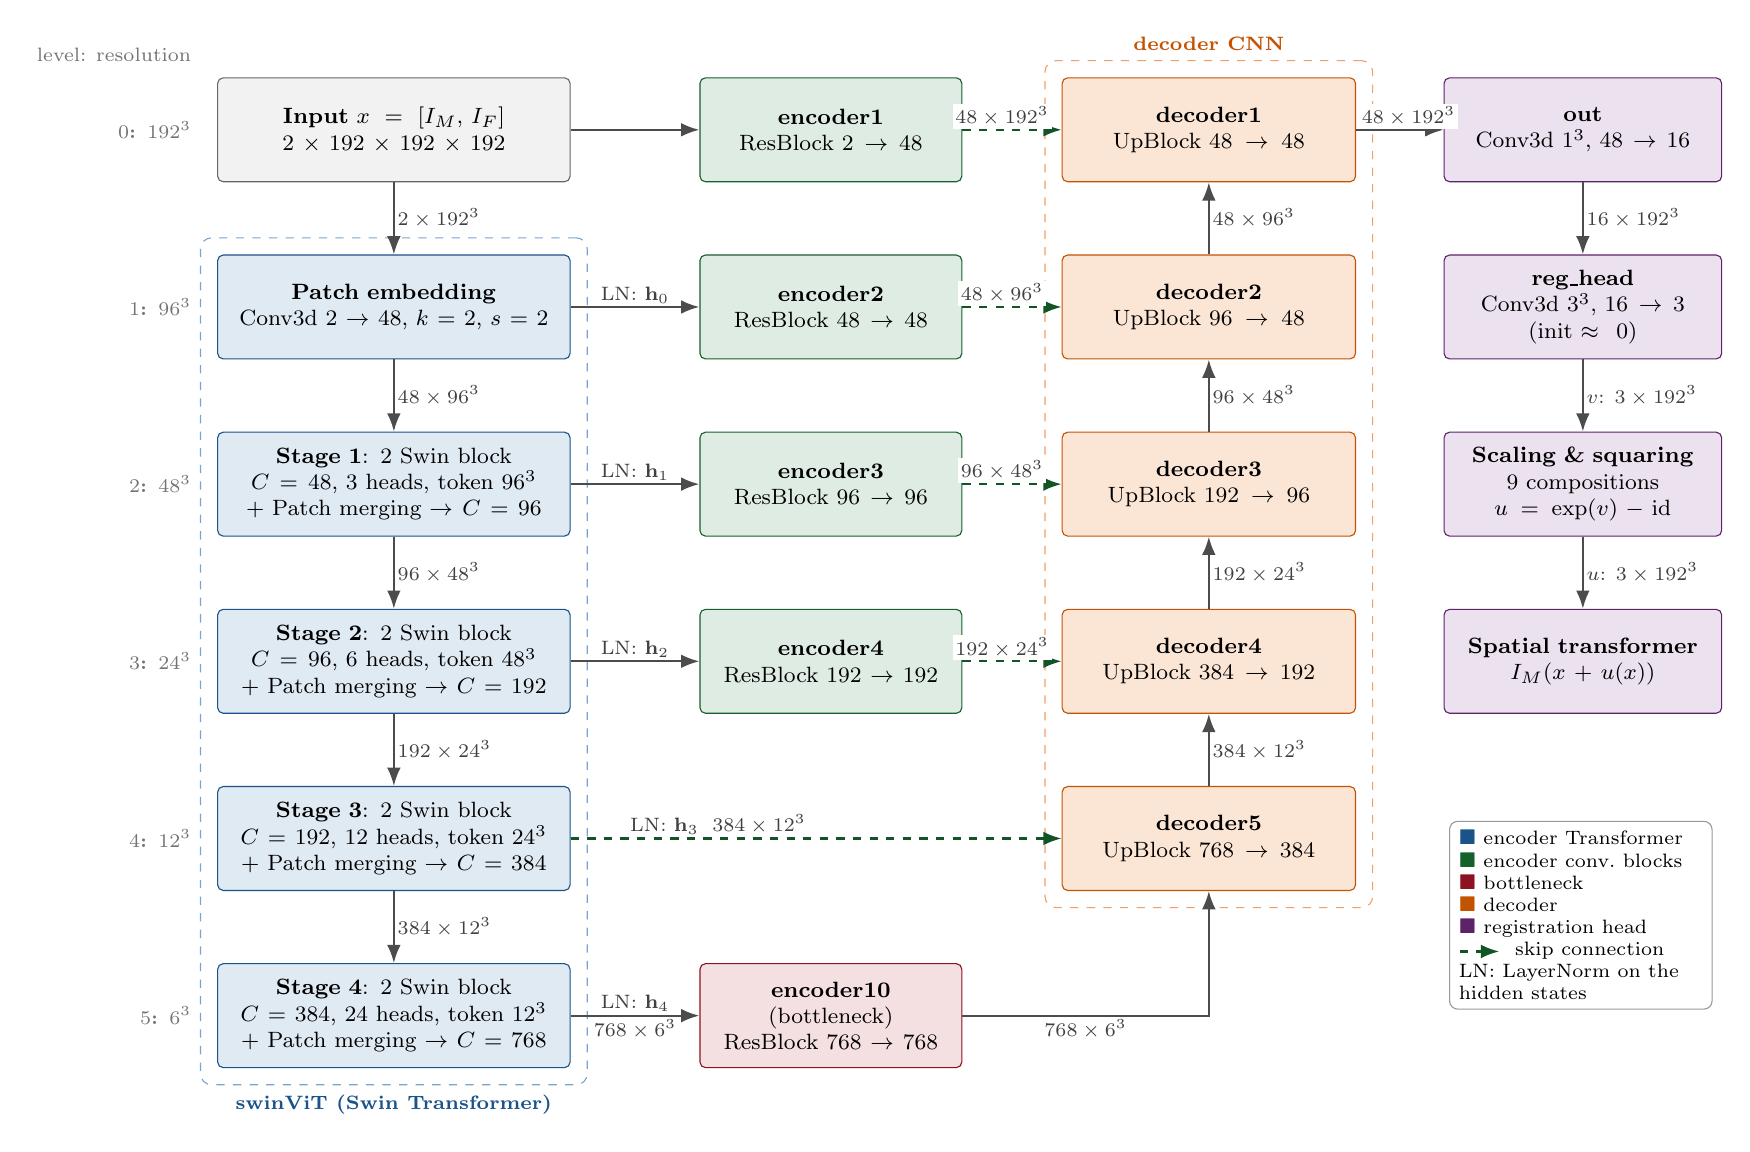
\begin{tikzpicture}[
  font=\footnotesize, >=Latex,
  box/.style={draw, rounded corners=2pt, align=center, minimum height=1.32cm, inner sep=2.5pt},
  swin/.style={box, fill=swinc!14, draw=swinc!80!black, text width=4.3cm},
  cnn/.style={box, fill=cnnc!14, draw=cnnc!80!black, text width=3.15cm},
  dec/.style={box, fill=decc!16, draw=decc!85!black, text width=3.55cm},
  bott/.style={box, fill=botc!14, draw=botc!80!black, text width=3.15cm},
  head/.style={box, fill=headc!14, draw=headc!80!black, text width=3.35cm},
  io/.style={box, fill=black!5, draw=black!60, text width=4.3cm},
  shp/.style={font=\scriptsize, fill=white, inner sep=1pt, text=black!75},
  arr/.style={->, thick, black!70},
  skip/.style={->, thick, dashed, cnnc!70!black}
]
\def\dy{2.25}
\def\xa{0}
\def\xb{5.55}
\def\xc{10.35}
\def\xd{15.1}

\foreach \L/\r in {0/{192^3},1/{96^3},2/{48^3},3/{24^3},4/{12^3},5/{6^3}} {
  \node[font=\scriptsize\bfseries, text=black!55, anchor=east] at (-2.45,-\L*\dy) {$\L$: $\r$};
}
\node[font=\scriptsize, text=black!55, anchor=east, align=right] at (-2.45,0.95) {level: resolution};

\node[io] (in) at (\xa,0) {\textbf{Input} $x=[I_M,\,I_F]$\\ $2\times192\times192\times192$};
\node[swin] (pe) at (\xa,-1*\dy) {\textbf{Patch embedding}\\ Conv3d $2\to48$, $k=2$, $s=2$};
\node[swin] (s1) at (\xa,-2*\dy) {\textbf{Stage 1}: 2 Swin block\\ $C=48$, 3 heads, token $96^3$\\ + Patch merging $\to C=96$};
\node[swin] (s2) at (\xa,-3*\dy) {\textbf{Stage 2}: 2 Swin block\\ $C=96$, 6 heads, token $48^3$\\ + Patch merging $\to C=192$};
\node[swin] (s3) at (\xa,-4*\dy) {\textbf{Stage 3}: 2 Swin block\\ $C=192$, 12 heads, token $24^3$\\ + Patch merging $\to C=384$};
\node[swin] (s4) at (\xa,-5*\dy) {\textbf{Stage 4}: 2 Swin block\\ $C=384$, 24 heads, token $12^3$\\ + Patch merging $\to C=768$};

\node[cnn] (e1) at (\xb,0) {\textbf{encoder1}\\ ResBlock $2\to48$};
\node[cnn] (e2) at (\xb,-1*\dy) {\textbf{encoder2}\\ ResBlock $48\to48$};
\node[cnn] (e3) at (\xb,-2*\dy) {\textbf{encoder3}\\ ResBlock $96\to96$};
\node[cnn] (e4) at (\xb,-3*\dy) {\textbf{encoder4}\\ ResBlock $192\to192$};
\node[bott] (e10) at (\xb,-5*\dy) {\textbf{encoder10}\\ (bottleneck)\\ ResBlock $768\to768$};

\node[dec] (d5) at (\xc,-4*\dy) {\textbf{decoder5}\\ UpBlock $768\to384$};
\node[dec] (d4) at (\xc,-3*\dy) {\textbf{decoder4}\\ UpBlock $384\to192$};
\node[dec] (d3) at (\xc,-2*\dy) {\textbf{decoder3}\\ UpBlock $192\to96$};
\node[dec] (d2) at (\xc,-1*\dy) {\textbf{decoder2}\\ UpBlock $96\to48$};
\node[dec] (d1) at (\xc,0) {\textbf{decoder1}\\ UpBlock $48\to48$};

\node[head] (out) at (\xd,0) {\textbf{out}\\ Conv3d $1^3$, $48\to16$};
\node[head] (rh) at (\xd,-1*\dy) {\textbf{reg\_head}\\ Conv3d $3^3$, $16\to3$\\ (init $\approx0$)};
\node[head] (ss) at (\xd,-2*\dy) {\textbf{Scaling \& squaring}\\ 9 compositions\\ $u=\exp(v)-\mathrm{id}$};
\node[head] (st) at (\xd,-3*\dy) {\textbf{Spatial transformer}\\ $I_M(x+u(x))$};

\draw[arr] (in) -- node[shp, right] {$2\times192^3$} (pe);
\draw[arr] (in) -- (e1);
\draw[arr] (pe) -- node[shp, right] {$48\times96^3$} (s1);
\draw[arr] (s1) -- node[shp, right] {$96\times48^3$} (s2);
\draw[arr] (s2) -- node[shp, right] {$192\times24^3$} (s3);
\draw[arr] (s3) -- node[shp, right] {$384\times12^3$} (s4);

\draw[arr] (pe) -- node[shp, above] {LN: $\mathbf{h}_0$} (e2);
\draw[arr] (s1) -- node[shp, above] {LN: $\mathbf{h}_1$} (e3);
\draw[arr] (s2) -- node[shp, above] {LN: $\mathbf{h}_2$} (e4);
\draw[arr] (s4) -- node[shp, above] {LN: $\mathbf{h}_4$} node[shp, below] {$768\times6^3$} (e10);
\draw[skip] (s3) -- node[shp, above, pos=0.3] {LN: $\mathbf{h}_3$ \;$384\times12^3$} (d5);

\draw[skip] (e1) -- node[shp, above, pos=0.4] {$48\times192^3$} (d1);
\draw[skip] (e2) -- node[shp, above, pos=0.4] {$48\times96^3$} (d2);
\draw[skip] (e3) -- node[shp, above, pos=0.4] {$96\times48^3$} (d3);
\draw[skip] (e4) -- node[shp, above, pos=0.4] {$192\times24^3$} (d4);

\draw[arr] (e10.east) -| node[shp, pos=0.25, below] {$768\times6^3$} (d5.south);
\draw[arr] (d5) -- node[shp, right] {$384\times12^3$} (d4);
\draw[arr] (d4) -- node[shp, right] {$192\times24^3$} (d3);
\draw[arr] (d3) -- node[shp, right] {$96\times48^3$} (d2);
\draw[arr] (d2) -- node[shp, right] {$48\times96^3$} (d1);
\draw[arr] (d1) -- node[shp, above, pos=0.6] {$48\times192^3$} (out);
\draw[arr] (out) -- node[shp, right] {$16\times192^3$} (rh);
\draw[arr] (rh) -- node[shp, right] {$v$: $3\times192^3$} (ss);
\draw[arr] (ss) -- node[shp, right] {$u$: $3\times192^3$} (st);

\begin{scope}[on background layer]
  \node[fit=(pe)(s4), draw=swinc!60, dashed, rounded corners=4pt, inner sep=6pt, label={[font=\scriptsize\bfseries, text=swinc!80!black]below:swinViT (Swin Transformer)}] {};
  \node[fit=(d5)(d1), draw=decc!60, dashed, rounded corners=4pt, inner sep=6pt, label={[font=\scriptsize\bfseries, text=decc!85!black]above:decoder CNN}] {};
\end{scope}

\node[draw=black!40, rounded corners=3pt, align=left, font=\scriptsize, anchor=north west, text width=3.1cm, fill=white] at (\xd-1.7,-3.9*\dy) {
\textcolor{swinc!80!black}{$\blacksquare$} encoder Transformer\\
\textcolor{cnnc!80!black}{$\blacksquare$} encoder conv.\ blocks\\
\textcolor{botc!80!black}{$\blacksquare$} bottleneck\\
\textcolor{decc!85!black}{$\blacksquare$} decoder\\
\textcolor{headc!80!black}{$\blacksquare$} registration head\\
\tikz[baseline=-0.5ex]\draw[skip] (0,0)--(0.5,0); \ skip connection\\
LN: LayerNorm on the hidden states};
\end{tikzpicture}
\end{document}
